\chapter{Wstęp}

Retusz zdjęć jest dzisiaj elementem rzeczywistości. Znaczna cześć otaczających nas reklam, okładki gazet i czasopism, zdjęcia zamieszczane w portalach internetowych i mediach społecznościowych, wszystkie one zostały zmodyfikowane, by trafić i spodobać się większemu gronu osób. Już nawet zakłady fotograficzne oferują lekki retusz zdjęć wykonanych do np. dyplomu, dowodu osobistego czy prawa jazdy \cite{retusz}. Tym samym, weryfikacja czy zdjęcie które oglądamy jest oryginałem, czy może zostało \textit{poprawione}, jest tak trudna. \\

Łatwość wykonania zmian na zdjęciach zawdzięczamy cyfryzacji zdjęć(pierwszy zapis zdjęcia cyfrowego - rok 1957 \cite{hist}) oraz coraz lepszemu oprogramowaniu do ich obróbki(luty 1990 - premiera pierwszej wersji Adobe Photoshop \cite{hist}). Historia tego zjawiska sięga jednak wcześniej. Przykładem niech będzie opisana w książce David Kinga \cite{stl} historia fotografii(patrz rysunek \ref{fig:stalin}) wykonanej 1915 roku na Syberii. W oryginale można zobaczyć 15 osób, dwadzieścia cztery lata później, w albumie wydanym na okoliczność sześćdziesiątych urodzin Józefa Stalina, na tej \textit{samej} fotografii widać już tylko 9 osób.
\begin{figure}[h!]
	\centering
	\subfloat{{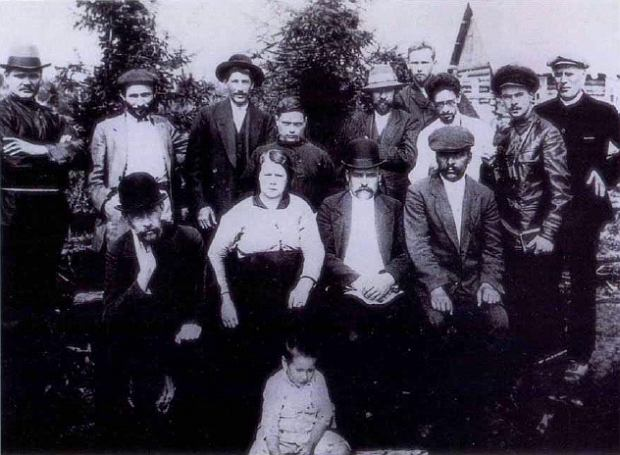
\includegraphics[width=6cm]{org.jpg} }}
	\qquad
	\subfloat{{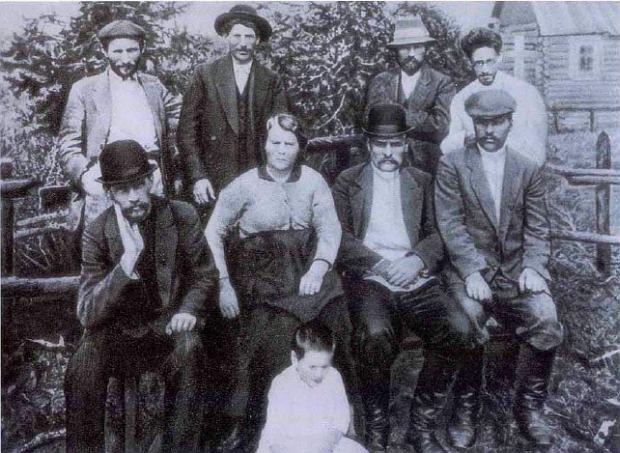
\includegraphics[width=6cm]{ret.jpg} }}
	\caption{Oryginalna fotografia wykonana w 1915 roku na Syberii oraz jej zmieniona wersja z albumu wydanego 1939 roku}
	\label{fig:stalin}
\end{figure}

Motywacją do napisania pracy był wykład wygłoszony w ramach kursu \textit{Metody głębokiego uczenia}, przez prowadzącego - mgr inż. Kamila Szyca, w poprzednim, zimowym semestrze(2019/2020), przybliżający sieci GAN oraz artykuł dotyczący sztucznego generowania twarzy \cite{gan}. Ważnym elementem zarówno wykładu jak i przywołanego artykuł jest fakt że zadanie generacji nowych treści(zdjęć twarzy) zostało określone jako łatwiejsze w stosunku do zadania oceny czy dane zdjęcie jest retuszowane czy nie. \\

Celem pracy jest zaproponowanie autorskiego rozwiązania do detekcji manipulacji zdjęć w postaci modelu sieci głębokiej. W ramach pracy nad tym zagadnieniem zostanie również przygotowany model maszyny wektorów nośnych, oraz model sieci głębokiej, opartej o rozwiązanie transferu wiedzy, tak by porównać efektywność zaproponowanych rozwiązań. \\

Praca została podzielona na sześć rozdziałów w następujący sposób. Rozdział pierwszy jest wstępem wprowadzającym w tematykę pracy. Rozdział drugi dotyczy szeroko-pojmowanego uczenia maszynowego i jego elementów zastosowanych w niniejszej pracy. Rozdział trzeci przybliża naukowe osiągnięcia i prace o tematyce podobnej do opisywanej - detekcji manipulacji zdjęć. W rozdziale czwartym postawione zostają pewne założenia metodologiczne co do samej pracy, w tym te dotyczące wyboru zbiorów danych, sposobu przeprowadzania eksperymentów i sposobu ich oceny. Rozdział piąty przedstawia szczegółowe implementacje wybranych klasyfikatorów oraz uzyskane przez nie wyniki. Całość tego rozdziału zakończona jest zestawieniem i omówienie uzyskanych rezultatów. Szóstym, ostatnim rozdziałem pracy jest podsumowanie, które to opisuje w jaki sposób zostały wypełnione założenia postawione niniejszej pracy, oraz kreśli w jaki sposób można by ją w dalszej części rozwijać.
